\documentclass[journal]{IEEEtran}

% correct bad hyphenation here
\hyphenation{op-tical net-works semi-conduc-tor}

\usepackage{amsmath}
\usepackage{amssymb}
\usepackage{bm}
\usepackage{booktabs}
\usepackage{float}
\usepackage{subcaption}
\usepackage{hyperref}
\usepackage{svg}
\newcommand{\bx}{\bm{x}}
\newcommand{\by}{\bm{y}}
\newcommand{\btheta}{\bm{\theta}}

\DeclareMathOperator{\expectation}{\mathbb{E}}
\DeclareMathOperator*{\argmin}{argmin}

\begin{document}

\title{Lecture summarization using sequential models}

\author{Mayank Mishra (2016EE30506), Tarun Kumar Yadav (2016CS10359)}

% make the title area
\maketitle

\begin{abstract}
Most online courses are very long and don't offer notes which makes it difficult for the students to take notes. We solve this problem by learning a sequential model trained on the video lectures. Learning to store information over extended time intervals is difficult using RNNs because of vanishing gradient problems. This makes it difficult to train vanilla RNNs. These problems are resolved by modern sequential models like LSTMs and GRUs. We train a Convolutional LSTMs on the given problem since the input to an LSTM cell is an image.

\end{abstract}

\section{Problem formulation}
Basically we have the task of identifying whether the current frame should be saved (recorded) or not. We have labelled data for the given problem. This task is posed as a distribution matching problem. The goal is to learn a non-linear mapping from the space of video frames $X$ to the space $Y$ of binary labels. We assume that such a transformation exists that takes an image $\bx_i \in X$ to its corresponding label $\by_i \in Y$. This problem can be cast into learning the parameters $\btheta \in \Theta$ that minimize the Kullback-Leibler divergence between the true distribution $q (\by | \bx)$ and the estimated distribution $p_{\btheta} (\by | \bx)$.

\begin{equation}
	\label{KL}
	\begin{aligned}
		D_{KL} \left[ q (\by | \bx) || p_{\btheta} (\by | \bx) \right] = \expectation_q [\log q (\by | \bx)] - \expectation_q [\log p_{\btheta} (\by | \bx)]
	\end{aligned}
\end{equation}
where $\bx$ denotes a frame.

Minimizing \eqref{KL} with respect to $\btheta$ is equivalent to minimizing the second term on the right hand side since the first term is independent of $\btheta$. The final objective reduces to:

\begin{equation}
	\label{objective}
	\begin{aligned}
		\btheta ^ * & = \argmin_{\btheta} - \expectation_q [\log p_{\btheta} (\by | \bx)]
		\\
		& = \argmin_{\btheta} \expectation_q [- \by \log h_{\btheta} (\bx) - (1 - \by) \log (1 - h_{\btheta} (\bx))]
	\end{aligned}
\end{equation}

using $p_{\btheta} (\by | \bx) = h_{\btheta} (\bx) ^ {\by} (1 - h_{\btheta} (\bx)) ^ {1 - \by}$, where $h(\bx)$ is given by $h_{\btheta} (\bx) = p_{\btheta} (\by = 1 | \bx)$.

Minimizing the KL will definitely converge since KL between two probability distributions is lower bounded by zero, with the KL being zero when the density functions for both the distributions are equal at all points in their domain.

The result is the familiar logistic regression problem with the Cross Entropy loss function \eqref{objective}. Theoretically, this can be solved by any function parametrized by $\btheta$. We use neural networks for the realization of this function.

\section{Convolutional LSTMs}
We use the convolutional LSTM architecture that can be used for classification, regression etc. LSTMs are simple temporal models. Convolutional LSTMs only differ from LSTMs in the sense that their basic operations are convolution operations.

\begin{equation}
	\label{conv_lstm}
	\begin{aligned}
		i_t = & \sigma(W_{xi} * x_t + W_{hi} * h_{t-1} + W_{ci} \circ c_{t-1} + b_i)
		\\
		f_t = & \sigma(W_{xf} * x_t + W_{hf} * h_{t-1} + W_{cf} \circ c_{t-1} + b_f)
		\\
		c_t = & f_t \circ C_{t-1} + i_t \circ tanh(W_{xc} * x_t + W_{hc} * h_{t-1} + b_c)
		\\
		o_t = & \sigma(W_{xo} * x_t + W_{ho} * h_{t-1} + W_{co} \circ c_{t} + b_o)
		\\
		h_t = & o_t \circ tanh(c_t)
	\end{aligned}
\end{equation}

\section{Experiments and results}
\subsection{Simple LSTM learned on embeddings of images}
We tried to learn the embeddings of the given images using simple autoencoders. These embeddings were then used to train a simple LSTM. However, the LSTM failed to learn anything. We tried to increase the model capacity by increasing number of layers and making it a 3-layered stacked LSTM. However, the model overfitted and trivially learned to remember the training data but failed to generalize to unseen test data.

\subsection{Convolutional LSTM on raw images}
We tried to learn a 3-layered convolutional LSTM on raw images. All images were resized to (240, 320, 3) where 3 is the number of channels in the image (RGB channels). The model performance is as shown in Table \ref{tab: conv}.

\subsection{Convolutional LSTM with CNN and attention with preprocessed images}
The raw images were pre-processed making them (240, 320, 6) where 6 is the number of channels in the images. We computed diff (refer Fig. \ref{fig: diff}) and optical flow using 2 consecutive images. The raw images were also passed through a Canny edge detector and the corresponding edge maps were obtained (refer Fig. \ref{fig: canny}). The images thus became 6-channeled (RGB, diff, optical flow, edgemap). These 6-channeled images were used to train a 3-layered convolutional LSTM with a simple CNN (with shared parameters across temporal dimensions) at the output of each cell in the third layer. This CNN was followed by an attention layer. The model did not perform substantially better than the simple convolutional LSTM model as shown in Table \ref{tab: cnnconv}.

\subsection{Convolutional LSTM on Fourier transform}
We also tried to train a simple convolutional LSTM on the Fourier transform of the images (240, 320, 2) where 2 is the number of channels (magnitude and phase spectrum). However, the model failed to learn anything even on the training data as the loss did not converge.

\begin{figure*}[t]
	\centering

	\begin{subfigure}{0.49\textwidth}
		\centering
		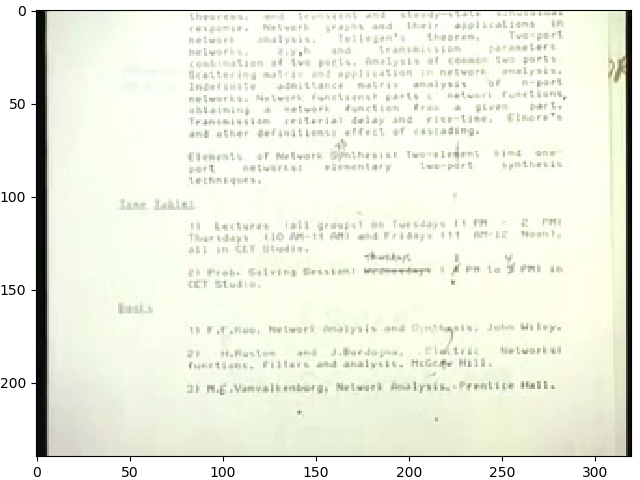
\includegraphics[height = 6cm]{Images/frame.png}
		\subcaption{Frame with label = 0}
	\end{subfigure}
	\hspace{1mm}
	\begin{subfigure}{0.49\textwidth}
		\centering
		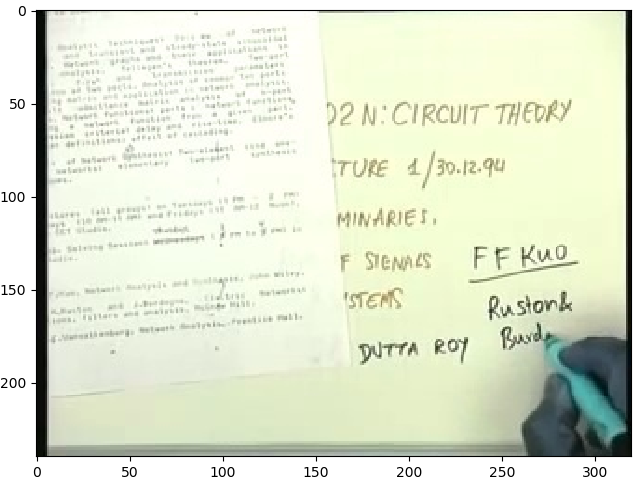
\includegraphics[height = 6cm]{Images/frame1.png}
		\subcaption{Frame with label = 1}
	\end{subfigure}

	\begin{subfigure}{0.49\textwidth}
		\centering
		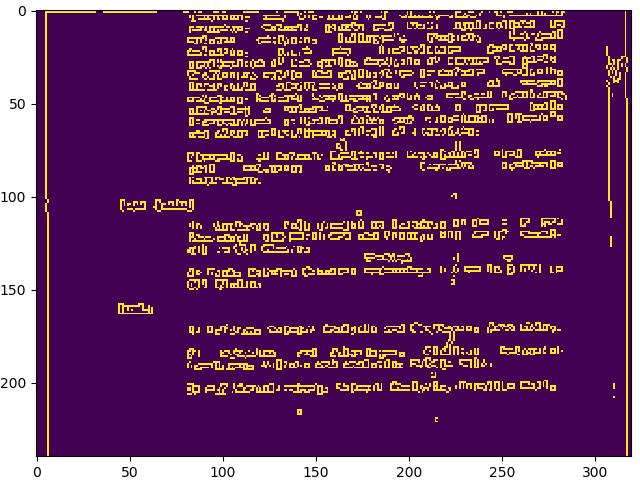
\includegraphics[height = 6cm]{Images/frameCanny.png}
		\subcaption{Frame with label = 0}
	\end{subfigure}
	\hspace{1mm}
	\begin{subfigure}{0.49\textwidth}
		\centering
		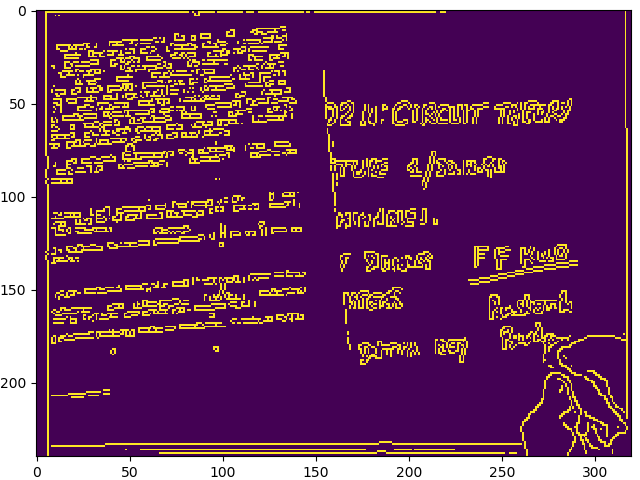
\includegraphics[height = 6cm]{Images/frameCanny1.png}
		\subcaption{Frame with label = 1}
	\end{subfigure}
	
	\caption{Frames with their edgemaps detected using Canny edge detector}
	\label{fig: canny}
\end{figure*}

\begin{figure*}[t!]
	\centering

	\begin{subfigure}{0.49\textwidth}
		\centering
		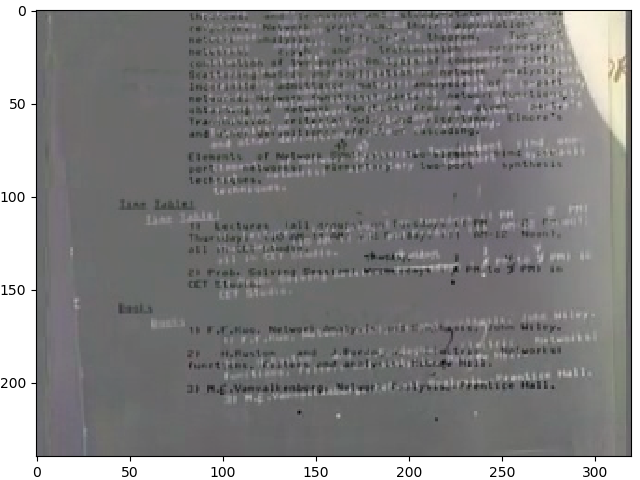
\includegraphics[height = 6cm]{Images/diff.png}
		\subcaption{when both frames have label = 0}
	\end{subfigure}
	\hspace{1mm}
	\begin{subfigure}{0.49\textwidth}
		\centering
		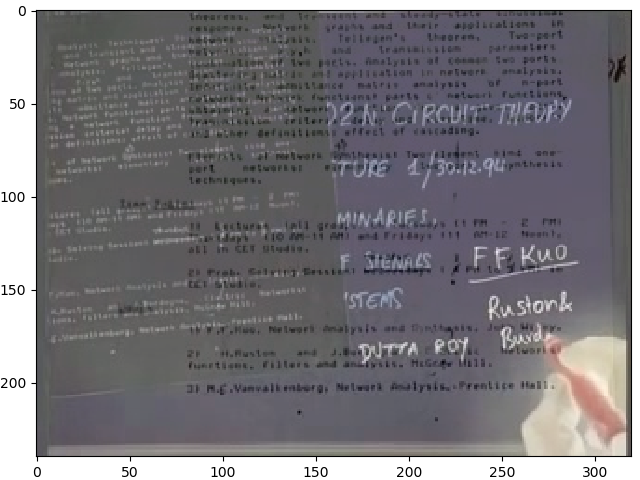
\includegraphics[height = 6cm]{Images/diff1.png}
		\subcaption{when one frame has label = 0 and one frame has label = 1}
	\end{subfigure}
	
	\caption{Diff of 2 consecutive images}
	\label{fig: diff}
\end{figure*}

\begin{table}[H]
	\caption{Metrics on simple convolutional LSTM}
	\centering
	\begin{tabular}{lll}
		\toprule
		Metric & Train set & Validation set
		\\
		\midrule
		Accuracy & 56.87 & 56.01
		\\
		F1 score & 59.84 & 58.73
		\\
		\bottomrule
	\end{tabular}
	\label{tab: conv}
\end{table}

\begin{table}[H]
	\caption{Metrics on convolutional LSTM with CNN at output with attention at the output of CNN}
	\centering
	\begin{tabular}{llll}
		\toprule
		Metric & Train set & Validation set
		\\
		\midrule
		Accuracy & 60.87 & 58.24
		\\
		F1 score & 62.94 & 61.26
		\\
		\bottomrule
	\end{tabular}
	\label{tab: cnnconv}
\end{table}

\begin{figure*}[h]
	\centering
	
	\begin{subfigure}{0.49\textwidth}
		\centering
		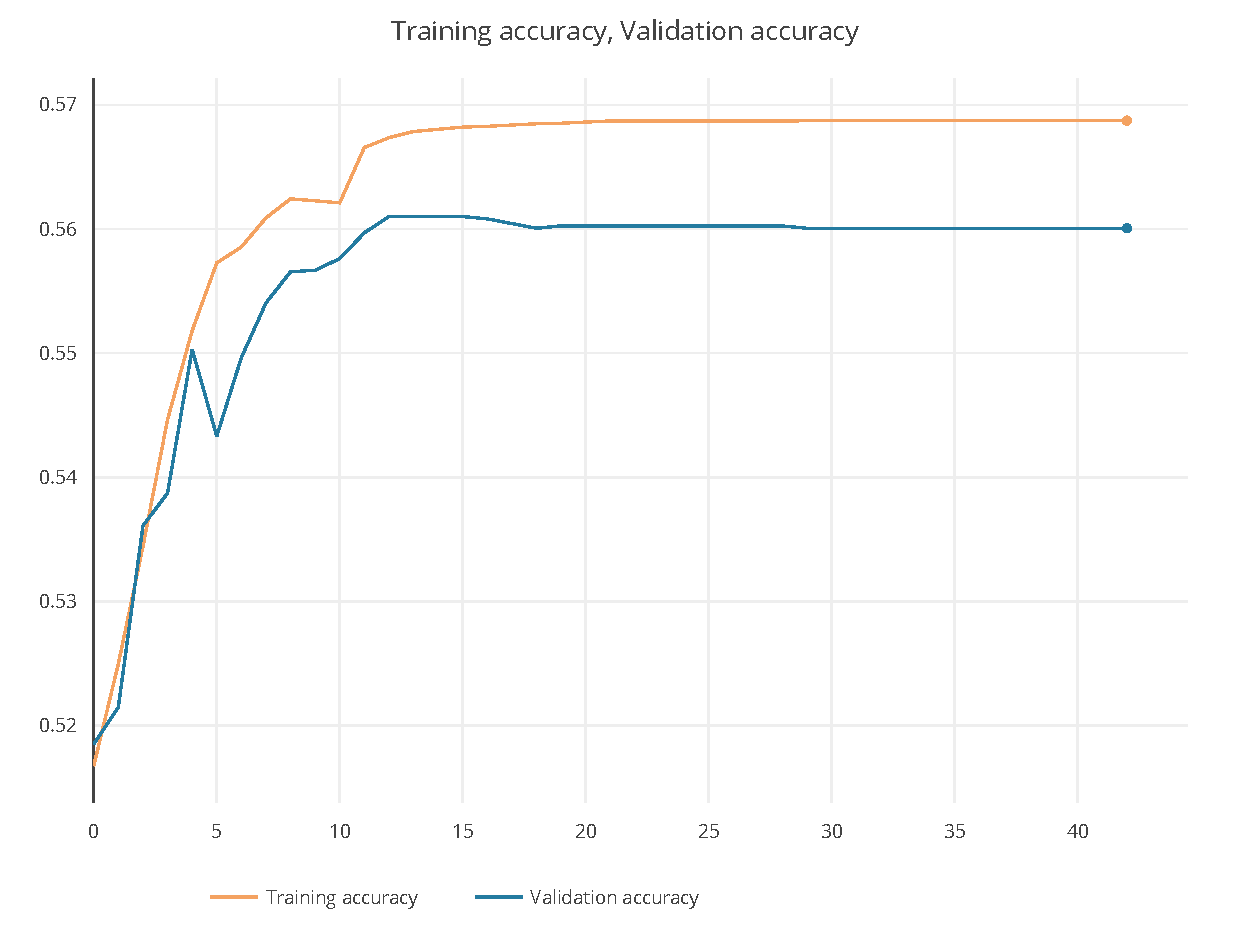
\includegraphics[height = 6cm]{Images/accuracy.pdf}
		\subcaption{Simple convolutional LSTM}
	\end{subfigure}
	\hspace{1mm}
	\begin{subfigure}{0.49\textwidth}
		\centering
		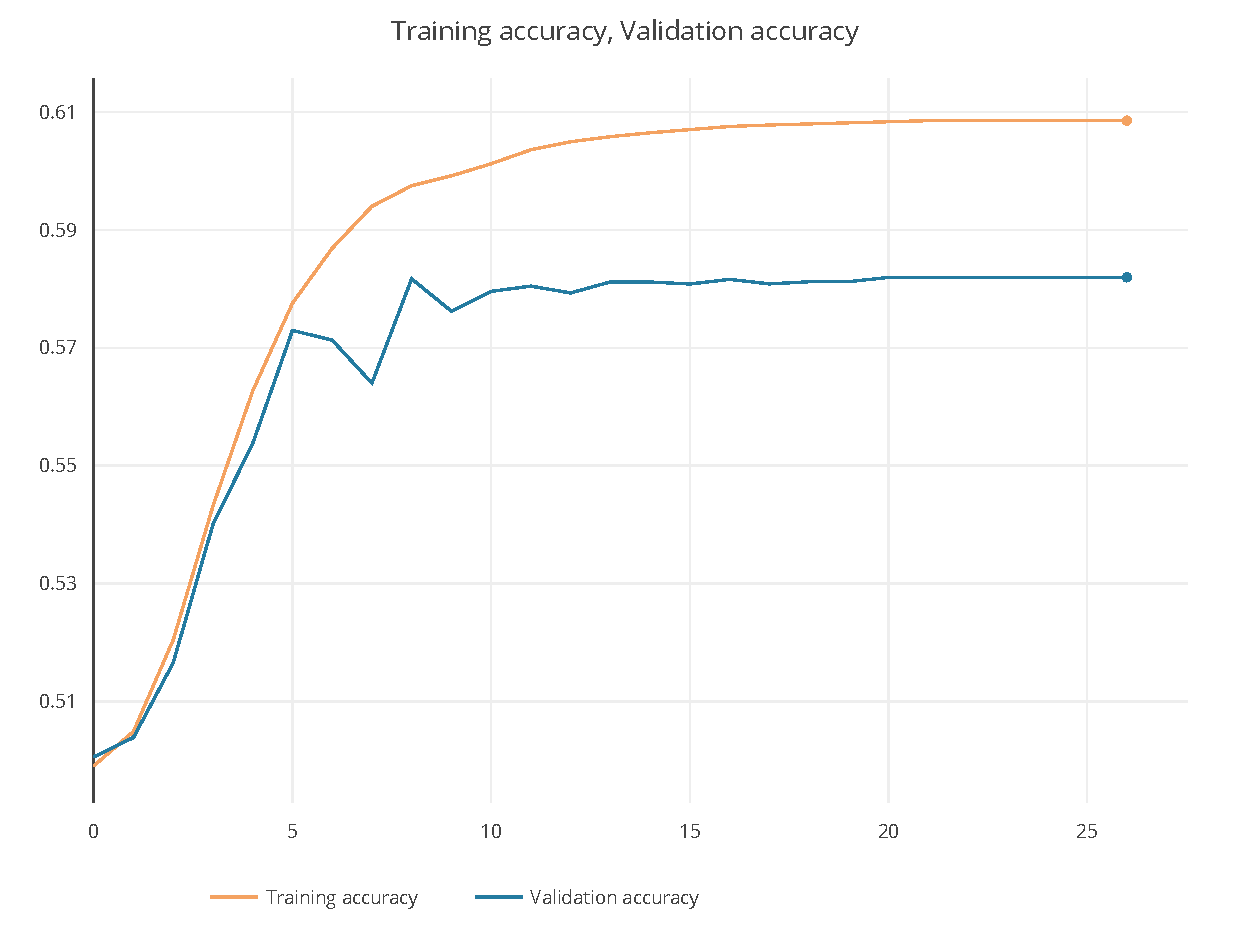
\includegraphics[height = 6cm]{Images/accuracy1.pdf}
		\subcaption{Convolutional LSTM with CNN and attention}
	\end{subfigure}
	
	\caption{Training and validation accuracy at each epoch}
\end{figure*}

\begin{figure*}[h]
	\centering

	\begin{subfigure}{0.49\textwidth}
		\centering
		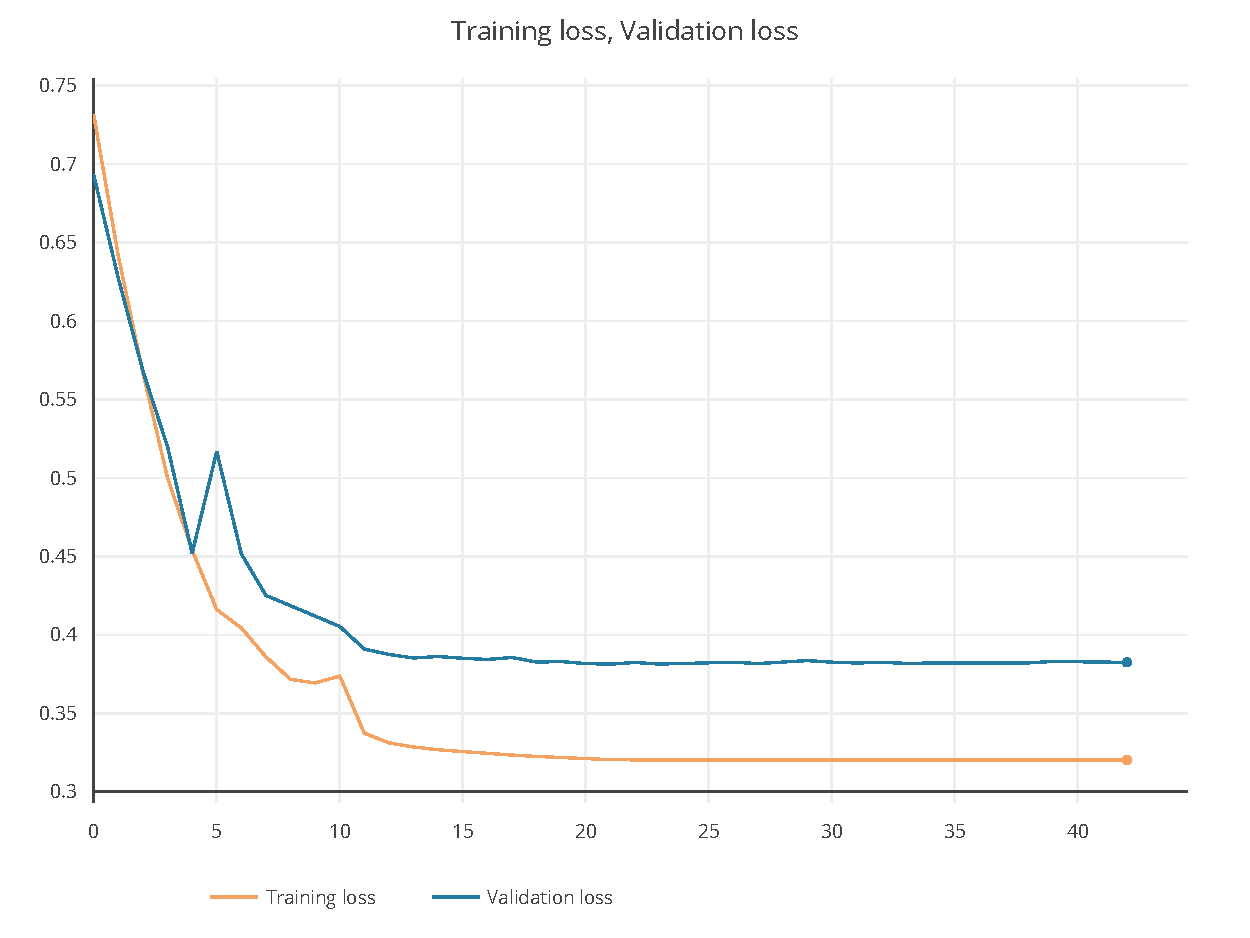
\includegraphics[height = 6cm]{Images/batchlosscurve.pdf}
		\subcaption{Simple convolutional LSTM}
	\end{subfigure}
	\hspace{1mm}
	\begin{subfigure}{0.49\textwidth}
		\centering
		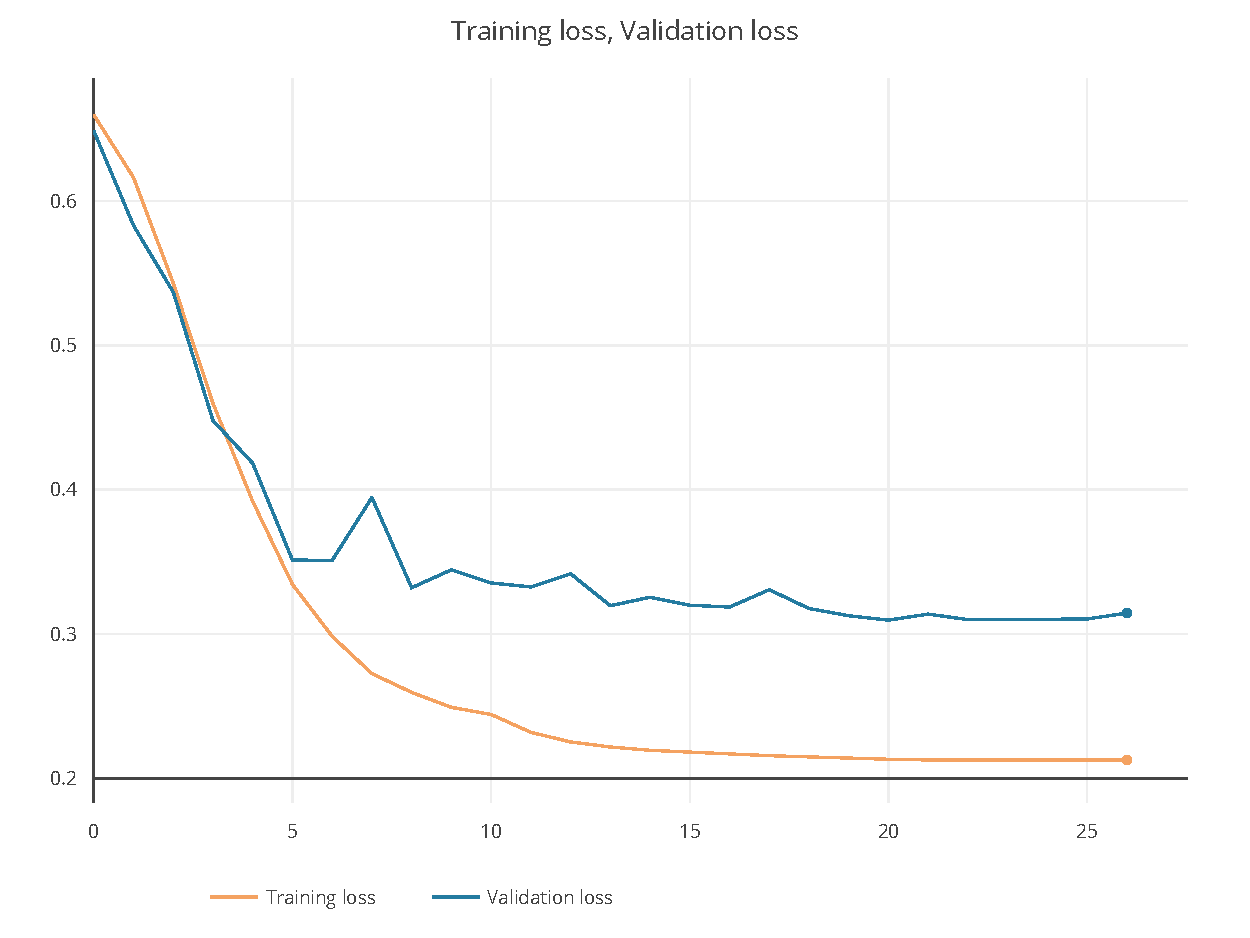
\includegraphics[height = 6cm]{Images/batchlosscurve1.pdf}
		\subcaption{Convolutional LSTM with CNN and attention}
	\end{subfigure}
	
	\caption{Training and validation loss at each epoch}
\end{figure*}

\begin{figure*}[h]
	\centering

	\begin{subfigure}{0.49\textwidth}
		\centering
		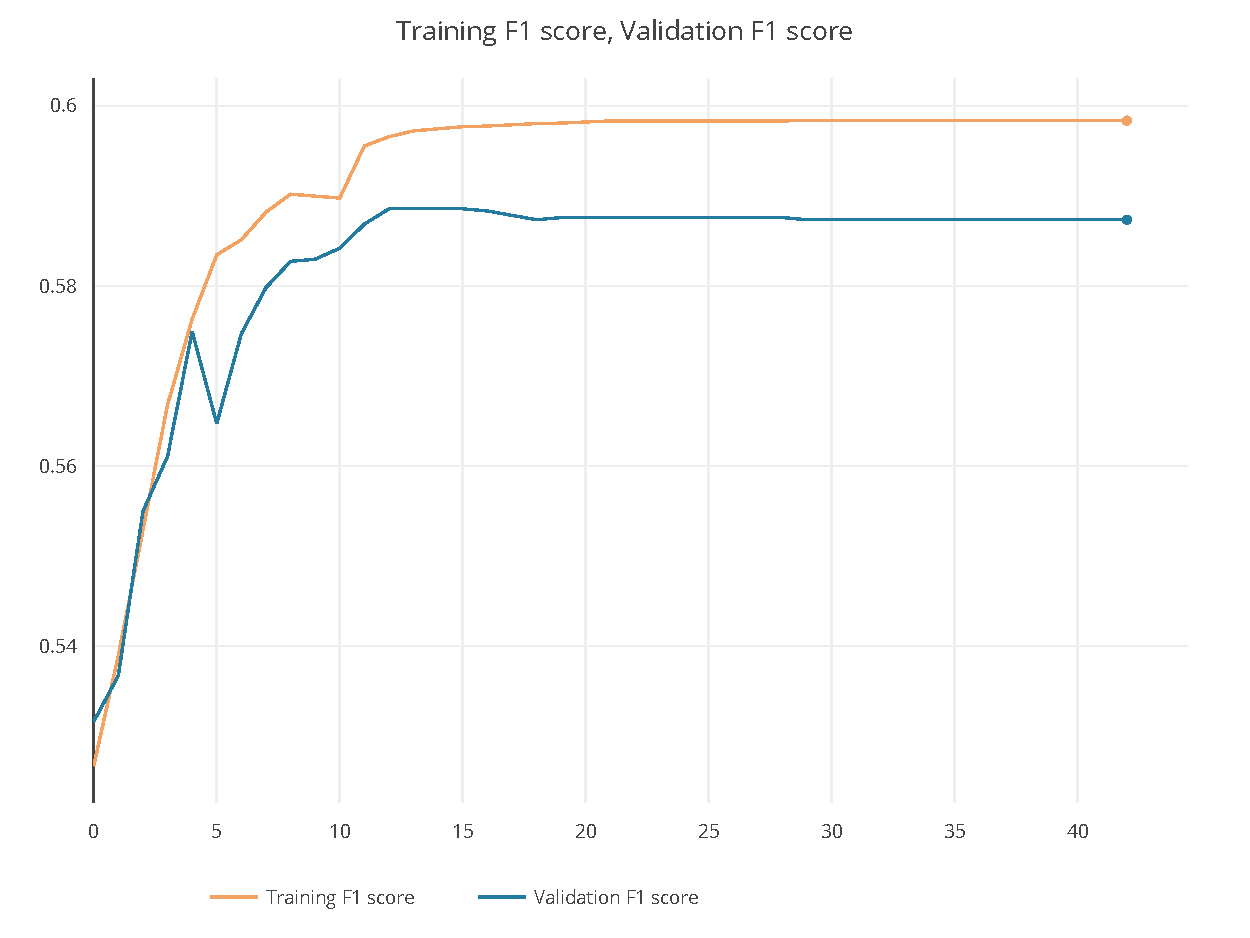
\includegraphics[height = 6cm]{Images/f1score.pdf}
		\subcaption{Simple convolutional LSTM}
	\end{subfigure}
	\hspace{1mm}
	\begin{subfigure}{0.49\textwidth}
		\centering
		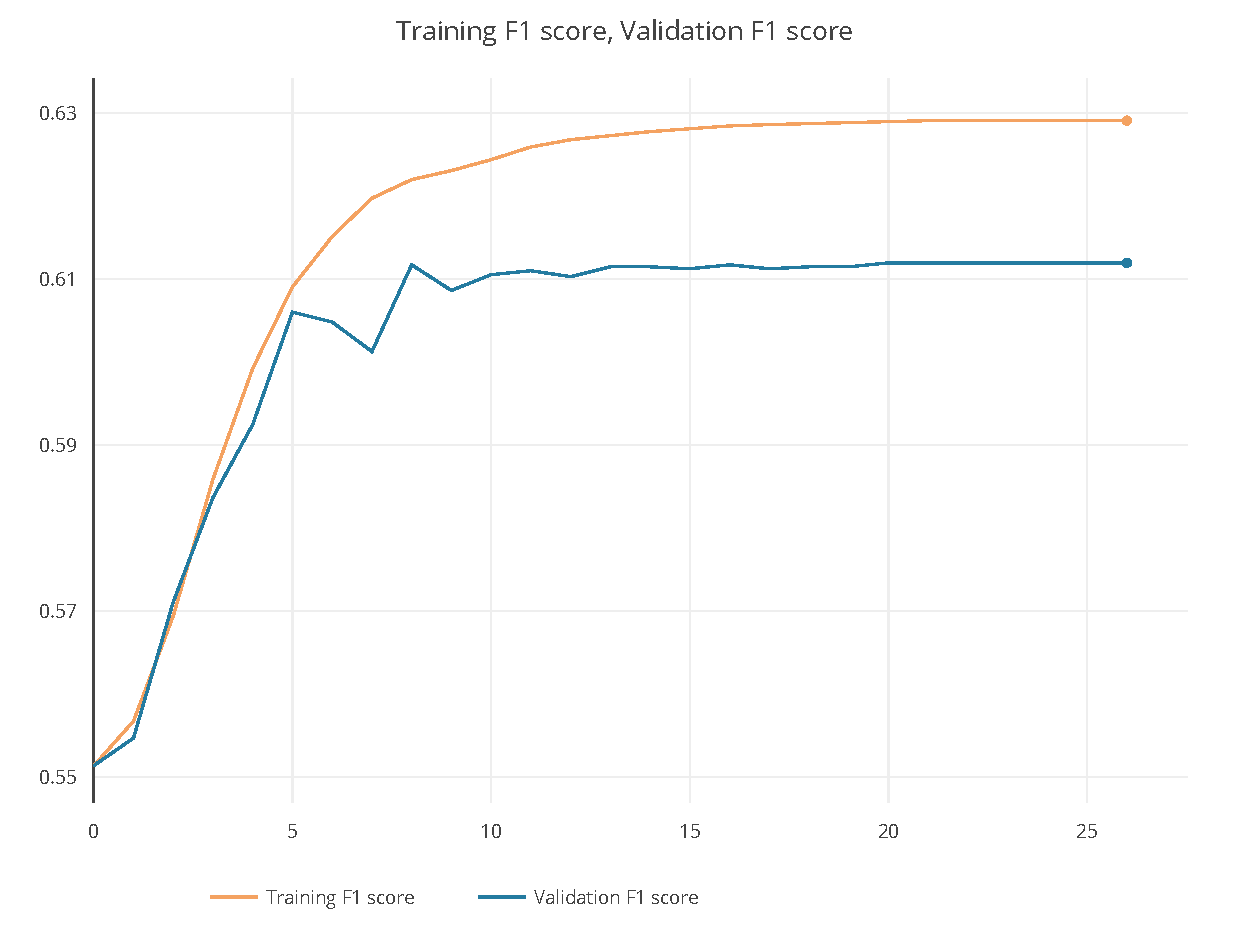
\includegraphics[height = 6cm]{Images/f1score1.pdf}
		\subcaption{Convolutional LSTM with CNN and attention}
	\end{subfigure}
	
	\caption{Training and validation F1 score at each epoch}
\end{figure*}

\begin{figure*}[h]
	\centering

	\begin{subfigure}{0.49\textwidth}
		\centering
		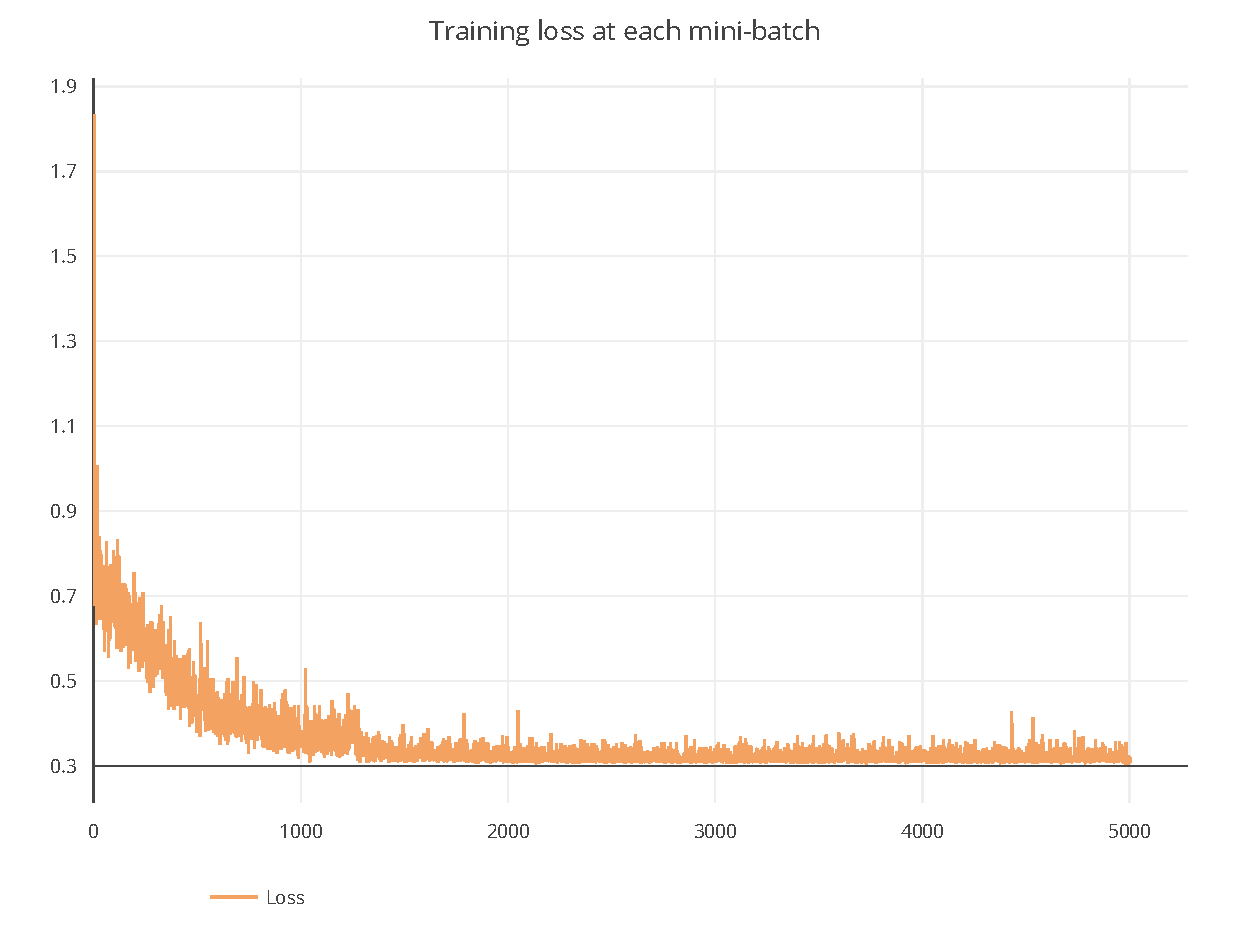
\includegraphics[height = 6cm]{Images/minibatchtrainloss.pdf}
		\subcaption{Simple convolutional LSTM}
	\end{subfigure}
	\hspace{1mm}
	\begin{subfigure}{0.49\textwidth}
		\centering
		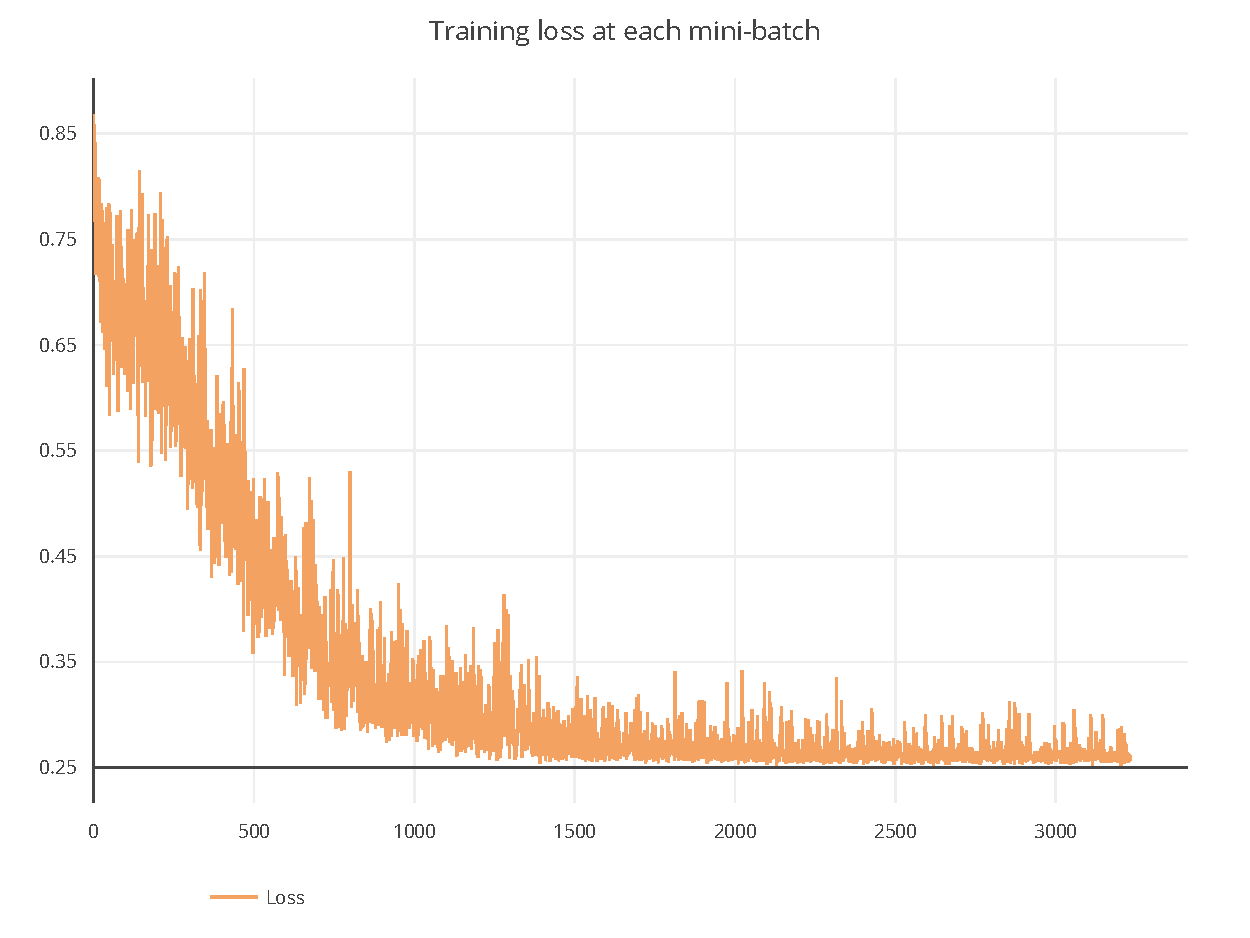
\includegraphics[height = 6cm]{Images/minibatchtrainloss1.pdf}
		\subcaption{Convolutional LSTM with CNN and attention}
	\end{subfigure}
	
	\caption{Training loss at each iteration}
\end{figure*}

\begin{figure*}[h]
	\centering

	\begin{subfigure}{0.49\textwidth}
		\centering
		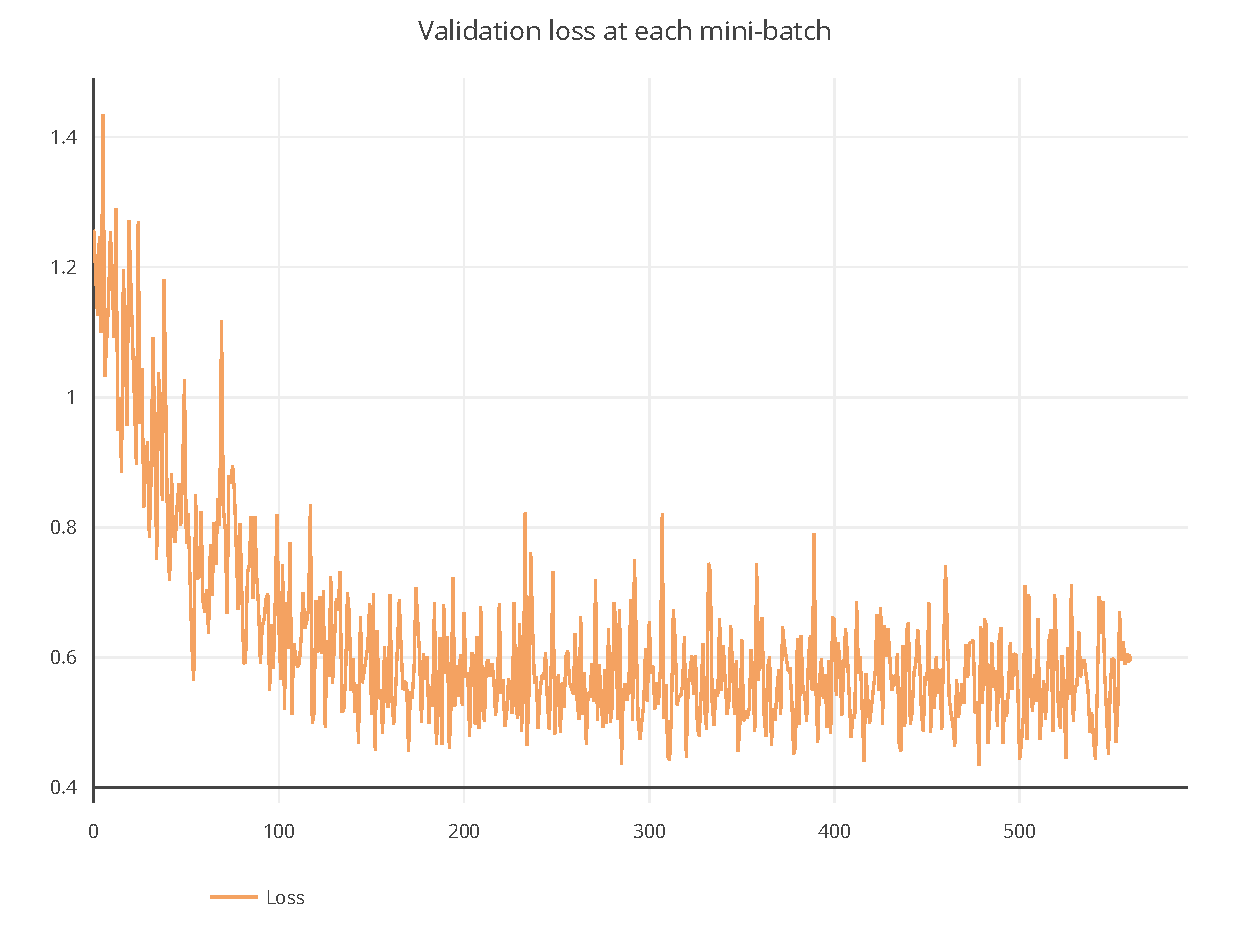
\includegraphics[height = 6cm]{Images/minibatchvalloss.pdf}
		\subcaption{Simple convolutional LSTM}
	\end{subfigure}
	\hspace{1mm}
	\begin{subfigure}{0.49\textwidth}
		\centering
		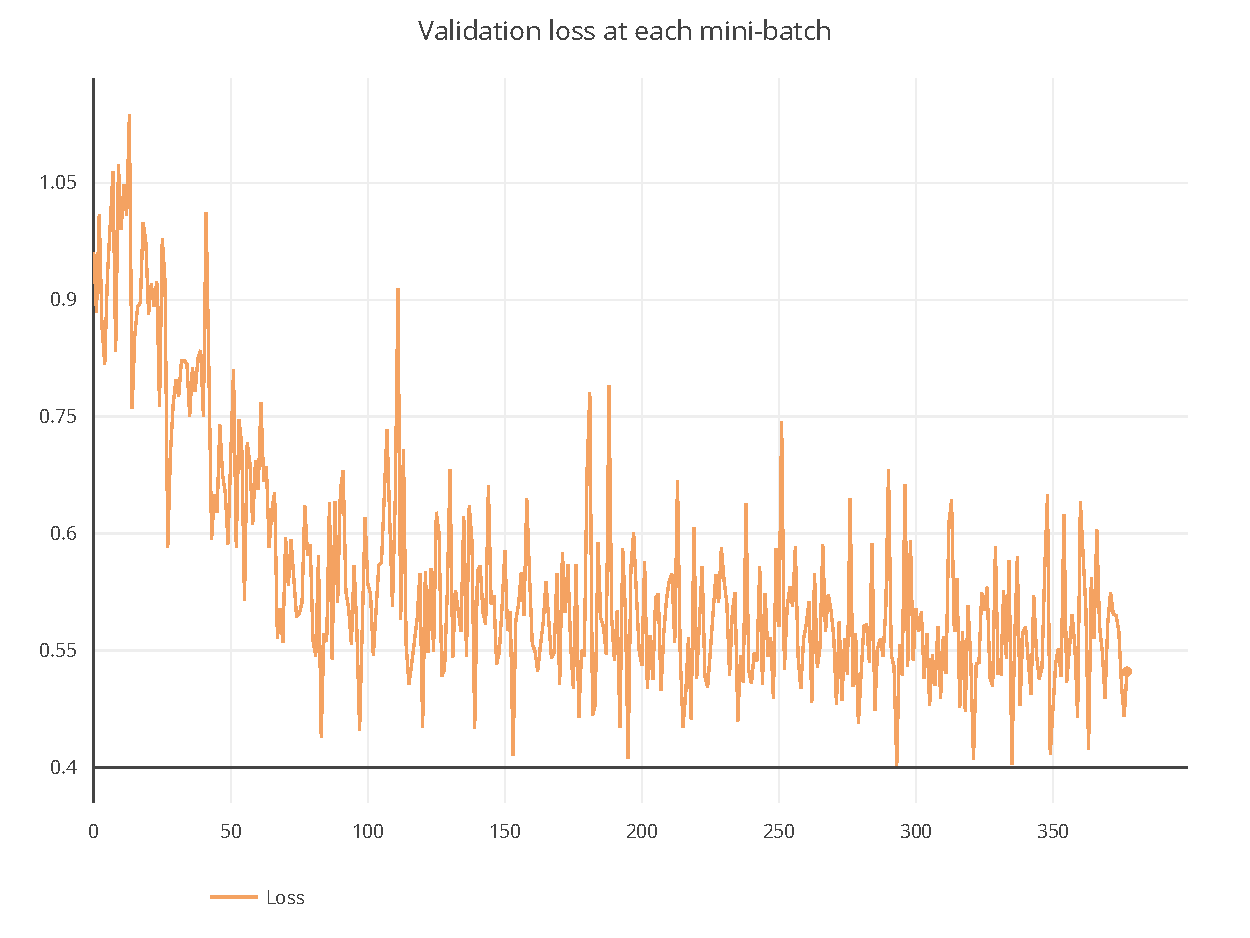
\includegraphics[height = 6cm]{Images/minibatchvalloss1.pdf}
		\subcaption{Convolutional LSTM with CNN and attention}
	\end{subfigure}
	
	\caption{Validation loss at each iteration}
\end{figure*}

\clearpage

\section{Conclusion}
In this work we train sequential models on NPTEL lectures and use it for lecture summarization. We try different model architectures. We also try pre-processing the data to impart som prior knowledge (prior knowledge is always helpful). We hypothesize that doing this kind of pre-processing should lead to better training as there is significant difference in the  edgemaps of images with label 0 and 1 (refer Fig. \ref{fig: canny}) and as the labels change the diff shows significant variation (refer Fig. \ref{fig: diff}).

\section*{Acknowledgement}
We would like to thank Dr. Prathosh A. P. for providing the dataset.

\bibliographystyle{ieeetr}

\end{document}
